\section{\textit{Layered Label Propagation}}

  A principal ideia dos algoritmos de \textit{Label Propagation} seguem um padrão comum. Estes algoritmos consistem num conjunto de iterações e no início é atribuído a cada vértice uma \textit{label} que representa o \textit{cluster} a que pertence. No início do algoritmo, cada vértice tem uma \textit{label} diferente. O critério de atribuição da \textit{label},a cada vértice, é o que diferencia os vários algoritmos de \textit{Label Propagation}. Um dos algoritmos mais conhecidos é o \textit{Standard Label Propagation}, em que a regra de atribuição da \textit{label} a um vértice é a \textit{label} que ocorrer mais frequentemente na sua vizinhança. 
  
  Uma outra variante, denominada \textit{Absolute Pott Model}, indica que a \textit{label} que é atribuída ao vértice é a que maximiza a seguinte equação: 
 
  \begin{center}
    \begin{equation}
      \label{apmeq}
      ki-\gamma(vi-ki)
    \end{equation}
  \end{center}    
  
  Sendo, $ki$ os vértices na vizinhança que têm a $label_i$ e $v_i$ todos os vértices que têm a $label_i$.
  Este algoritmo pode ser descrito da seguinte forma:
  
  \begin{algorithm}[H]
    \caption{\textit{Absolute Pott Model}}\label{apmalg}
    \begin{enumerate}
    \item Obter uma permutação do grafo.
    \item Iniciar todos os vértices atribuindo uma \textit{label} única e por $v_i=1$ para cada $label_i$ .
    \item Iterar sobre a permutação obtida e para todas as \textit{labels} na vizinhança de cada vértice ver qual é maximizada pela equação \ref{apmeq} e atribuir ao vértice essa \textit{label}. Decrementar $v_i$ para a \textit{label} antiga e incrementar o $v_i$ correspondente à nova \textit{label}.
    \end{enumerate}
  \end{algorithm}

  Ambos os algoritmos apresentados anteriormente têm alguns problemas. O \textit{Standard Label Propagation} tende a produzir um \textit{clusters} de grandes dimensões(contendo a maior parte dos vértices) e o \textit{Absolute Pott Model} tem o problema de não se saber à partida o valor ideal para $\gamma$.
  
  \subsection{Algoritmo de \textit{Layered Label Propagation}}
  Baseado no algoritmo \textit{Standard Label Propagation} surgiu o \textit{Layered Label Propagation}. Este algoritmo consiste no seguinte:
  
  \begin{algorithm}[H]
    \caption{\textit{Layered Label Propagation}}\label{llpalg}
    \begin{enumerate}
    \item Para cada iterações chamar o Algoritmo \ref{apmalg} tendo $gama$ valores compreendidos dentro do seguinte conjunto: $\{0\}\cup\{2^{{-}i},i=0,...,K\} $.
    \item Com o \textit{output} resultante da chamada ao Algoritmo \ref{apmalg}, ordenar os vértices de modo a que os que tenham a mesma \textit{label} fiquem próximos. Para vértices que estejam na mesma comunidade (têm a mesma \textit{label}) é mantida a sua ordem.
    \end{enumerate} 
  \end{algorithm}
  
  \paragraph{Exemplo} Para o grafo da Figura \ref{graph0llp} pode-se calcular 
de forma sequencial o Layered Label Propagation, para cada iteração $i$, 
começando por se fazer uma permutação($\pi_i$) dos vértices do grafo e itera-los 
por essa ordem. 
  
  \begin{figure}[H]
    \center
    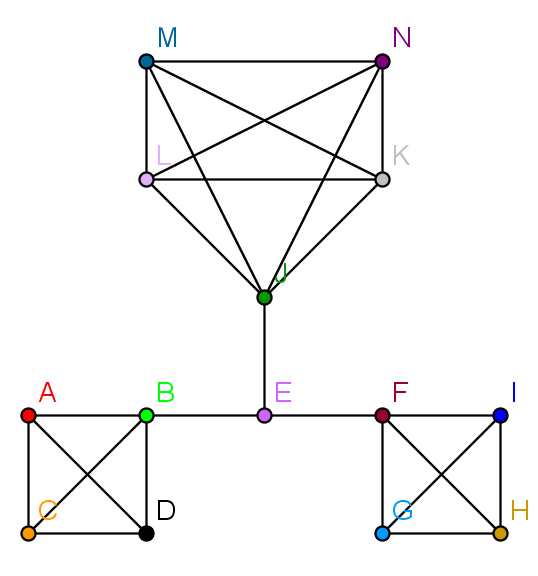
\includegraphics{graph_step0.png}
    \caption{Grafo de exemplo em que cada vértice foi-lhe atribuída uma \textit{label}(cor) inicial que é única.}
    \label{graph0llp}
  \end{figure}
  
  Neste contexto as \textit{labels} serão iteradas de forma a que seja dada uma maior importância à que o vértice tem e de seguida à que pertence ao vértice com menor ordem lexicográfica.

  Para $i=1$ admite-se que $\pi_1=$[N,H,M,B,J,L,G,D,K,E,I,F,C,A], $\gamma=1$(para facilitar) e que $v_i$=1 para todas as \textit{label}. Segundo o algoritmo \ref{apmalg} segue-se a iteração sobre $\pi_1$ e para cada vértice vê-se qual a \textit{label} que maximiza a Equação \ref{apmeq}. 
  %Nesta primeira iteração para qualquer vértice o resultado da equação \ref{apmeq} referente à sua \textit{label} não é o valor que maximiza porque $k_i=0$ e o mesmo acontece para as \textit{labels} que não se encontram na vizinhança, daí a omissão destes elementos. 
  \\[0.25cm]
  Exemplo para N:
  \begin{itemize}
   \item $label_n = k_n - \gamma ( v_n - k_n ) = 0 - 1 ( 1 - 0) = -1$
   \item $label_j = k_j - \gamma ( v_j - k_j ) = 1 - 1 ( 1 - 1) = 1$\\
   {\bf N fica com a \textit{label} de J.}
   \item $label_k = k_k - \gamma ( v_k - k_k ) = 1 - 1 ( 1 - 1) = 1$
   \item $label_l = k_l - \gamma ( v_l - k_l ) = 1 - 1 ( 1 - 1) = 1$ 
   \item $label_m = k_m - \gamma ( v_m - k_m ) = 1 - 1 ( 1 - 1) = 1$
  \end{itemize}
  Este cálculo é feito para todos os vértices pela ordem de $\pi_1$.  \\[0.25cm]
  \begin{figure}[H]
    \center
    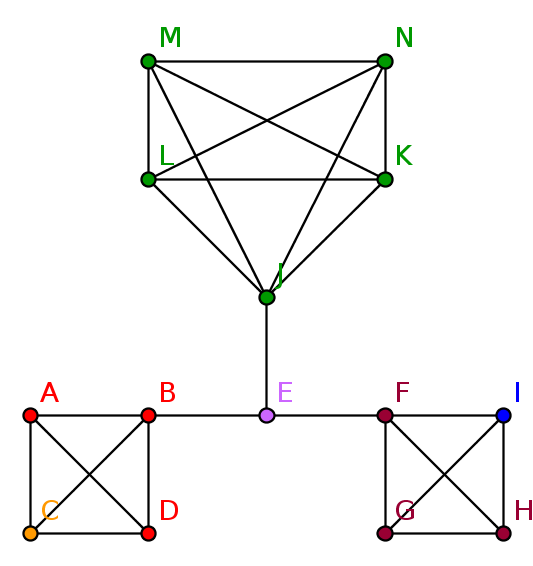
\includegraphics{graph_stepAtE.png}
    \caption{Grafo de exemplo a iterar $\pi_1$ em E}
    \label{graphEllp}
  \end{figure}
  
  Exemplo para E:
  \begin{itemize}
   \item $label_e = k_e - \gamma ( v_e - k_e ) = 0 - 1 ( 1 - 0) = -1$
   \item $label_a = k_a - \gamma ( v_a - k_a ) = 1 - 1 ( 3 - 1) = -1$
   \item $label_f = k_f - \gamma ( v_f - k_f ) = 1 - 1 ( 3 - 1) = -1$ 
   \item $label_j = k_j - \gamma ( v_j - k_j ) = 1 - 1 ( 5 - 1) = -3$\\
   {\bf E mantém a sua \textit{label}.}
  \end{itemize}
  
  No final deste percorrer $\pi_1$ o grafo irá ter 4 comunidades com está 
  apresentado na Figura \ref{graphfinalllp}.
  
  \begin{figure}[H]
    \center
    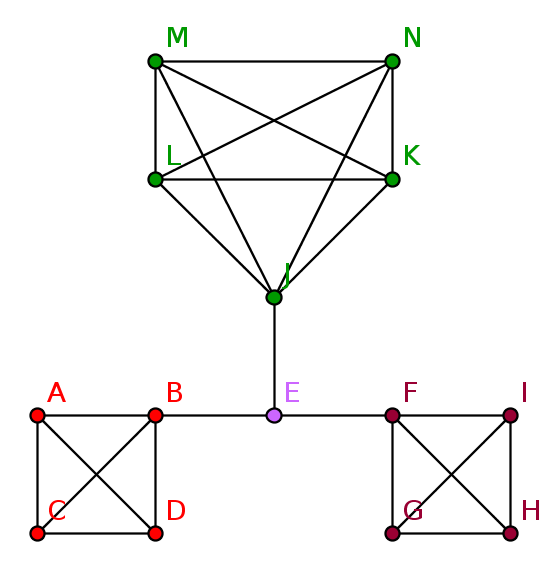
\includegraphics{graph_stepFinal.png}
    \caption{Grafo depois de iterar $\pi_1$ de acordo com o Algoritmo \ref{apmalg}.}
    \label{graphfinalllp}
  \end{figure}
  
  O algoritmo do \textit{Layered Label Propagation} após fazer o algoritmo de
  Absolute Pott Model reordena os vértices de acordo com a sua comunidade 
(mantendo a ordem dos vértices com a mesma comunidade) e volta a fazer este 
processo.

\subsection{Algoritmo de \textit{Layered Label Propagation} Distribuído}

O algoritmo apresentado anteriormente pode ser usado em grafos de grandes
dimensões em plataformas distribuídas. Contudo, existe algumas mudanças quanto 
à várias fases do algoritmo. 

  O facto de se estar a usar uma plataforma distribuídas e a ordem que os 
vértices são iterados tem alguma aleatoriedade então a fase de obtenção da 
permutação do vértices é garantida. Após a obtenção da permutação como o 
algoritmo \ref{apmalg} indica, apenas é necessário iterar sobre as 
\textit{labels} que estão na vizinhança. Contudo, é necessário haver uma fase 
de agregação para saber o $v_i$ correto em todos os vértices que têm uma 
determinada $label_i$ de modo a que o valor de $v_i$ não esteja desatualizado 
nas extremidades da comunidade. Para haver essa agregação do $v_i$ há a 
necessidade de cada vértice enviar para o representante da sua comunidade. O 
representante de uma comunidade tem de enviar de volta o valor atualizado de 
$v_i$.

O representante de uma comunidade pode ser um vértice qualquer, isto é, não 
tem de necessariamente pertencer à comunidade, isto permite evitar algumas 
situações que podiam a levar ao aumento da complexidade do algoritmo. Por 
norma, o representante de uma comunidade A é o vértice A.

Para resolver os problemas associados à resolução do algoritmo \textit{Layered 
Label Propagation} distribuído é proposto o algoritmo \ref{llpdistributed2}. 
Neste algoritmo o representante de uma determinada comunidade não precisa de 
pertencer a essa mesma comunidade e a resolução de ciclos é resolvida apenas 
parando o vértice, caso este tente mudar-se para a comunidade que esteve 
anteriormente. Para este algoritmo é necessário o uso de mensagens compostas 
por: vértice de origem(quem envia a mensagem), $label_i$ do vértice e $v_i$ 
conhecido da sua $label_i$. É ainda necessário que cada vértice tenha de ser 
composto por: a sua $label$ atual, a $label$ que teve antes de obter a $label$ 
atual e um valor booleano indicado se pode computar ou não uma nova $label$.

\begin{enumerate}
\begin{algorithm}
  \caption{\textit{Layered Label Propagation} Distribuído.} 
\label{llpdistributed2}
\begin{minipage}{\textwidth}
     \item Inicialização:
     \begin{enumerate}
      \item Iniciar cada vértice com a sua $label$ atual e anterior igual ao 
seu id. A booleana que impede o vértice de mudar de $label$ deve estar a false.
     \end{enumerate}
     \item 1º Passo - Enviar para a sua adjacência o valor de $vi$ atualizado
     \begin{enumerate}
      \item Se tiver recebido mensagem implica ter recebido um valor atualizado 
de $vi$, caso contrário o $vi$ é 1.
      \item Enviar para os seus vértices adjacentes informação acerca do 
vértice atual. 
     \end{enumerate}
     \item 2º Passo - Cálculo da nova $label$.
      \begin{enumerate}
	\item Verificar a booleana do vértice para ver se pode fazer este 
passo. Caso o vértice não possa fazer este passo, então a sua booleana é posta 
num estado em que se possa fazer um próximo 2º passo do algoritmo e envia-se 
para o seu representante\footnote{O representante é igual à $label$ que o 
vértice tem.} uma mensagem. Caso o vértice não possa fazer o passo pode-se 
parar o vértice.
	\item Calcular a formula \ref{apmeq} para as $labels$ que recebeu 
e para a sua $label$ atual.
	\item Verificar se a $label$ calculada é diferente da $label$ que o 
vértice tinha anteriormente. Caso a $label$ seja igual, meter a booleana num 
estado que impeça o vértice de calcular no próximo 2º passo. Caso a $label$ 
for diferente, então mudar as $labels$ ao vértice.
	\item Enviar para o seu representante indicando que está na sua 
comunidade e parar o vértice.
	\item Pode-se parar o vértice.
      \end{enumerate}
      \item 3º Passo - Cálculo de $vi$ nos representantes.
      \begin{enumerate}
       \item Calcular o novo $vi$ ($vi$ = o número de mensagens recebidas).
       \item Enviar para todos os vértices que lhe enviaram mensagem o novo $vi$
      \end{enumerate}
\end{minipage}
\end{algorithm}
\end{enumerate}

\clearpage

 \paragraph{Exemplo} \textit{Layered Label Propagation} distribuído, o  segundo 
o algoritmo \ref{llpdistributed2}, tendo em como grafo inicial o representado 
na 
Figura \ref{graph0llp}:

{\bf Fase de preparação:}\\
Todos os vértices ficam com uma $label$ única. 
\\[0.25cm]
{\bf \textit{Superstep} 0  (1º Passo do algoritmo):}
Os vértices não receberam mensagens, logo não precisam de atualizar o seu $v_i$.
Os vértices enviam para os seus adjacentes informação sobre a sua 
\textit{label} e com $v_i=1$.
\\[0.25cm]
{\bf \textit{Superstep} 1 (2º Passo do algoritmo):}
Os vértices recebem as mensagens enviadas pelos seus adjacentes e calculam a 
$label_i$ que é maximizada na sua vizinhança. Cada vértice envia uma mensagem 
para o seu representante.
\\[0.25cm]
{\bf \textit{Superstep} 2 (3º Passo do algoritmo):} Os vértices representantes 
de cada comunidade calculam o $v_i$ atualizado para a sua $label_i$ e devolvem 
para os seus membros.
\\[0.25cm]
{\bf \textit{Superstep} 3 (1º Passo do algoritmo):}
Os vértices recebem mensagens do representante, logo iram meter o seu $v_i$ 
igual ao que receberam.
Os vértices enviam para os seus adjacentes informação sobre a sua sua 
\textit{label} e com $v_i$ atual.
\\[0.25cm]
{\bf \textit{Superstep} 4 (2º Passo do algoritmo):}
Os vértices voltam a calcular a $label_i$ que é maximizada na sua vizinhança, 
contudo podem não a escolher. Caso a $label_i$ que maximize for a $label_i$ 
anterior que o vértice teve, então o vértice mantém a sua $label_i$ e não irá 
fazer o próximo 2º passo (porque a sua booleana que impede a sua computação foi 
posta a verdadeiro). Caso a $label_i$ não seja a $label_i$ anterior, o vértice 
pode mudar para essa comunidade. Em ambos os casos o vértice envia para o seu 
representante uma mensagem.
\\[0.25cm]
Repete-se os vários passos até que nenhum vértice mude no 2º passo do 
algoritmo. No final as comunidades serão as identificadas pela seguinte figura:

\begin{figure}[h]
  \center
  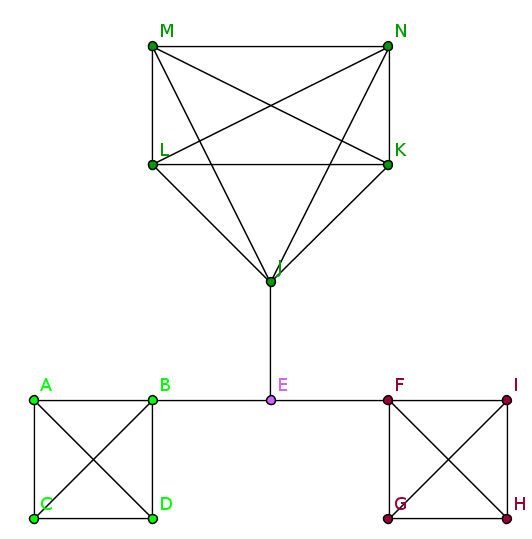
\includegraphics{graph1_end}
  \caption{Comunidades finais do grafo \ref{graph0llp} segundo o algoritmo de 
\textit{Layered Label Propagation} distribuído.}
\end{figure}
